\documentclass[10pt,
%superscriptaddress,
%groupedaddress,
%unsortedaddress,
%runinaddress,
%frontmatterverbose, 
%preprint,
%preprintnumbers,
%nofootinbib,
%nobibnotes,
%bibnotes,
 amsmath,amssymb,
 aps,prb, twocolumn
]{revtex4-2}


% Graphics and math
\usepackage{graphicx}
\usepackage{bm}
\usepackage{dcolumn}
\usepackage{physics}
\usepackage{soul}
\usepackage{dsfont}
\usepackage{xcolor} % for more colors
% Subfigures (compatible with REVTeX)
\usepackage[caption=false]{subfig}  
% Hyperlinks (must come last)
\usepackage[colorlinks=true,allcolors=blue]{hyperref}
\begin{document}

\newcommand{\id}{\mathds{1}}
\newcommand\sj[1]{ {\color{cyan} #1} } 
\newcommand\jm[1]{ {\color{magenta} #1} } 
\definecolor{mediumgreen}{HTML}{228B22} % forest green-ish
\newcommand\oz[1]{ {\color{mediumgreen} #1} } 

\title{Measurement Kick as a Scattering Event}

\author{Santiago Salazar Jaramillor}
\email{santiago.salazar-jaramillo@uni-konstanz.de}
\author{Jeff Maki}
\email{jeffrey.maki@uni-konstanz.de}

\author{Oded Zilberberg}
\email{oded.zilberberg@uni-konstanz.de}
\affiliation{Department of Physics, University of Konstanz, 78464 Konstanz, Germany}


\date{\today}

\begin{abstract}
    We develop a minimal model of a single measurement event between a qubit and a detector particle...
\end{abstract}

\maketitle

\section{Introduction}\label{sect:introduction}

\sj{Santiago comments/edits}, \jm{Jeff comments/edits}, \oz{Oded comments/edits}\\

\begin{itemize}
    \item Saving intro for the end.
\end{itemize}

The measurement problem is one of the most important unanswered questions in quantum mechanics. At the heart of the matter, is the collapse postulate \cite{wigner1995}, which introduces non-unitary stochastic jumps to the otherwise deterministic, unitary evolution predicted by the Schrödinger equation.

Already in 1932, John Von Neumann proposed an extension to the Copenhagen interpretation \cite{vonNeumann1932}, by adding the detector and its interaction with the target system to the Hamiltonian as quantum objects. 

Although this does not solve the underlying problem, it has resulted in novel effects such as non-projective, continuous measurements \cite{tamir013}, and weak value experiments \cite{aharonov1988, alonso2005}, providing a more general theory of measurement beyond collapse of the wave function. 

Quantum Point Contacts are charge detectors, \st{exhibiting quantized conductance} \cite{wharam1988, vanhouten1996,vanwees1988, tekman1991} capable of realizing such non-invasive measurements \cite{field1993}. Explain the working principle.

Experimental realizations and advantages of Quantum Point Contact. These studies evidence that QPCs have the potential to carry out both information processing and control protocols in a quantum computing setup.

 It has been shown that, the current flowing through QPCs becomes correlated to the state of the qubit \cite{gurvitz1996,  gurvitz1997, korotkov2001}.

Using the rate equation formalism, it has been shown that QPC measurements can achieve fine control over quantum dot systems \cite{ferguson2023, zilberberg2014} and are adequate detectors of coherent transport \cite{rech2011, zilberberg2019}. 

 What is missing from the rate equations that may be captured in single events. 

 Existing studies ... (\sj{Here we should look at Klaus Mølmer's work})

Therefore, it is desirable to study the effects of a QPC measurement on a qubit for a single event.

In this work, we develop a minimal model of a single measurement event between a qubit and a detector particle. Using exact diagonalization, together with a perturbative analysis and the ancilla paradigm, we find an optimal regime for measurement and identify the mechanisms behind entanglement generation.

\section{Hamiltonian and Measurement Setup}\label{sect:model}

\begin{itemize}
    \item Introduce the ``unraveled Hamiltonian'' in Eq.\eqref{eq:qpc_dd_H}, sketched in Figs.\ref{fig:h_model} and \ref{fig:bloch_sphere}, and define all quantities.
    \item The decoupled energies are Eq.\eqref{eq:decoupled_energies}.
    \item Composite initial state is a product state Eq.\eqref{eq:initial_state}.
    \item Initial condition for QPC is a wavepacket \eqref{eq:gauss_wavepacket}.
    \item Initial state for qubit ensures orbit is within the x-z plane.
    \item We keep our treatment purely Hamiltonian and unitary, so observables like entropy are readily available.

%     Eq.\eqref{eq:gauss_wavepacket}. \sj{Allows well defined measurements according to} \cite{vonNeumann1932}.
%     \item Explain notation.
%     % \item In order to have a well defined measurement in the von Neumann sense, we need the wave packet in Eq.\eqref{eq:gauss_wavepacket} for the QPC particle, which introduces an interaction time window. \jm{@Santiago: more details on conditions of wavepacket for measurement. We are missing a step between initial conditions and measurement.}
%     \item We solve it using ED + perturbation, details in \ref{app:numerical_setup}.
%    \item \sj{Explicitly mention the ranges/values for parameters.}

%    \item \sj{Mention that the initial condition of the qubit has to be carefully selected to make sensible comparisons}.
\end{itemize}

\begin{align}\label{eq:qpc_dd_H}
    \hat{H} = -J \sum_{j=1}^N \hat{c}^{\dagger}_{j+1}\hat{c_{j}} - \omega \hat{d}_1 \hat{d}_0  + g \hat{d}^{\dagger}_{1}\hat{d}_{1}\hat{c}^{\dagger}_{b+1}\hat{c}_{b}  + \text{h.c.}
\end{align}

\begin{align}\label{eq:decoupled_energies}
    & E(k) = -J \cos{k0} \\
    & \epsilon_\pm = \pm \omega
\end{align}

\begin{align}\label{eq:initial_state}
    \ket{\Psi} = \ket{\psi}\otimes(\alpha_0\ket{0}+\beta_0\ket{1})
\end{align}

\begin{align}\label{eq:gauss_wavepacket}
    &\ket{\psi} = \left(\frac{1}{\pi \Delta^2}\right)^{1 / 4} e^{-\frac{1}{2 \Delta^2}\left(x_j-x_c\right)^2+i k_0\left(x_j-x_c\right)} \ket{\vec{j}}
\end{align}

 \begin{figure} 
  \centering
  \subfloat[]{%
    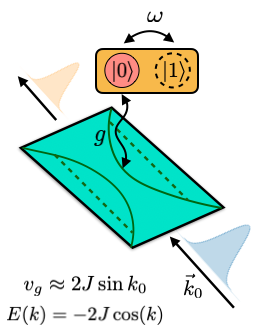
\includegraphics[width=0.55\linewidth]{Figures/model_sketch.png}
    \label{fig:h_model}
  }\\[1em] 
  \subfloat[]{%
    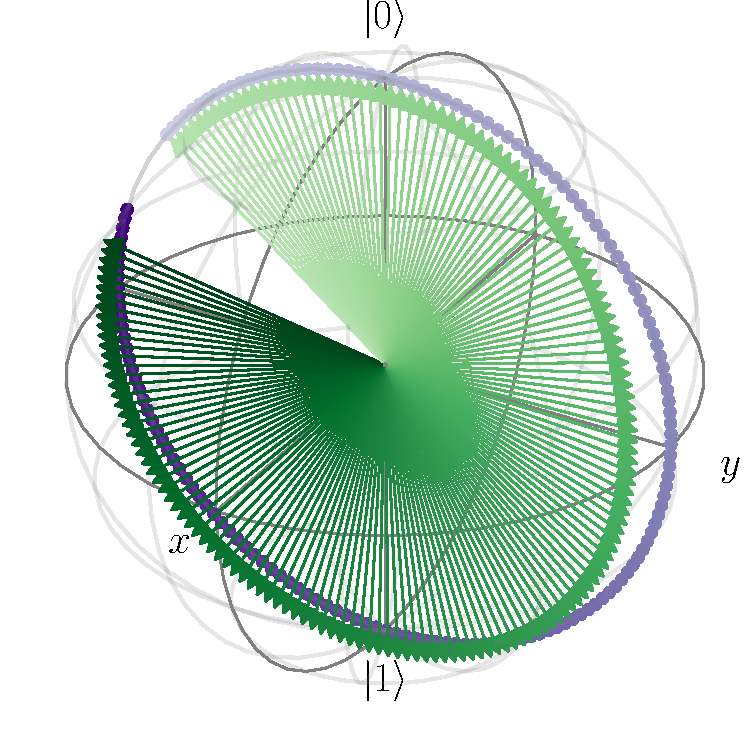
\includegraphics[width=0.55\linewidth]{Figures/bloch_orbits.pdf}%
    \label{fig:bloch_sphere}
  }
  \caption{(a) Diagram of the model in Eq.\eqref{eq:qpc_dd_H}, the QPC particle is represented as a Gaussian wavepacket and the qubit as a 2-level system. (b) Bloch sphere trajectories for the qubit \sj{I should include the theta and phi angles in the figure to also show the notation}. The free evolution corresponds to the purple dots and the QPC influenced one to the green arrows}\label{fig:backaction_intuit}
\end{figure}

\section{Comparison to Other Models}\label{sect:comparison_to_others}

\begin{itemize}
    \item Wavepacket allows for the notion of a measurement time ($\delta \tau = \Delta(k_0)/v_g$) in terms of its spread which is dependent on $k_0$. 
    
    \item Comparing $k_0$ to the Rabi frequency allows us to define different regimes.
    
    \item In the limit of a slow (quasi-static) qubit (with respect to $k_0$), measurement according to von Neumann. 

    \item VN is a unitary Hamiltonian approach for a single measurement event, where the detector is a free wave-packet and the the qubit's dynamics are deprecated during the interaction window.
    
    \item VN produces an entangled state, where the momentum of the detector is coupled to the system's measured observable.

    \item Hence, measurement is done by reading out the detector state with a projection, which yields partial information on the entangled observable. Through this, VN provides a platform for weak-measurements. 
    
    \item An extension of VN to multiple measurement kicks in a QPC is found in K \cite{korotkov1999} and G \cite{gurvitz1997}.
    
    \item In K and G, it is assumed that, i) the qubit is slow enough to be considered constant over a single kick, ii)  the detector and system are weakly coupled. These are the same assumptions as VN.

    \item These assumptions alow a formulation where the readout observable is the current through the QPC.

    \item \st{K and G obtain Bloch-like (classical) equations of motion for the qubit density matrix in terms of the QPC transmission rate.}
    
    \item The current becomes dependent on qbit's occupation and agrees with Landauer (Fermi's golden rule zeroth order effect).  \sj{do we include the equaion here?}

    \item The backaction on the qubit is manifested as dephasing (exponential decay of coherences) and a slow down of the Rabi frequency.

    \item in the quasi-static limit, our results should be consistent with VN and KG, we also expect such behavior in our model.
    
    \item  In addition, we expect a phase gain since the interaction and free Hamiltonian's do not commute (we break non-demolition) \cite{siddiqi2024}.

    \item In the opposite limit of fast qubit (Floquet), we expect decoupled dynamics as the qubit's oscillations are too fast to be affected by a single kick and the QPC wavepacket will experience the qubit as a constant potential.
    
    \item However, in the intermediate (coherent) regime, the oscillations of the QPC will be important for a single kick.

    \item Here, one can expect that $k_0 / \omega$ will play a role in the measurement outcome, but its difficult to get a priori intuition as its is not a commonly discussed.

    \item We can explore all of these regimes by tuning the Rabi frequency and $v_g$ in our model Eq.\eqref{eq:qpc_dd_H}.

    \item  We can solve the exact dynamics with ED (details in \ref{app:numerical_setup}).

    \item \sj{Notice that, our model is equivalent to measurement without readout  so there is no projection applied on the QPC.}

    \item ED allows us to get the exact backaction from the reduced density matrix on the qubit, which we can contrast to von Neumann/KG. 
    
    % Similar to scattering
    % \item in the limit of fast qubit, they become decoupled.
    % \item 

    
    % \item Discuss various limits of the model Weak vs strong interaction, Slow vs fast QPC, slow vs fast qubit.
    % \item \sj{Note that we explicitly break non-demolition so we expect a phase gain}.
    % \item How our model matches K \cite{korotkov1999} and G \cite{gurvitz1997}. State their two key assumptions.
    % \item Conclude section with how our model encapsulates all these limits, translate their assumptions into our language.
    % \item In the following section, we \sj{discuss the backaction on the qubit from ED and provide an analytical toy model}.
    % % \item Contrast our Hamiltonian with \cite{gurvitz1997,korotkov1999}. Typically, a QPC is modeled as two leads (a source and a drain) connected by a single site. Since current is the readout observable, single electron events are coarse grained over, resulting in classic-like rate equations for the density matrix elements \cite{gurvitz1996}. \jm{@Santiago. I think this goes later. We need a bridge between what we did and others.}
    % % \item Discuss the wave function Ansatz?
    % % \item The current through the QPC depends on the occupation in the qubit, following with Landauer's $T = (J- p_0\Omega)^2$. Which is Fermi's golden rule i.e zeroth order approximation. 
    % % \item We can go beyond their 2 main assumptions (The qubit does not oscillate during a single measurement kick and one stays withing the weak measurement regime), because we are including the coherent qubit oscillations. We consider the fully opened QPC case for simplicity. \jm{@Santiago, I think this should go later}
    % % \item We calculate the time evolution using exact diagonalization. Discussion of the numerical setup is in Appendix \ref{app:numerical_setup}.
\end{itemize}


\section{Results}\label{sect:Results}

\subsection{Measurement Backaction}\label{sect:backaction}

\begin{itemize}
    
    \item With ED, we obtain the exact qubit density matrix, and the Bloch angles $\theta, \phi$ at all times. Details in \ref{app:numerical_setup}.

    \item The backaction after measurement, is shown in Fig.\ref{fig:backaction_k0} with the phase gain $\Delta \phi$ Fig.\ref{fig:delta_phi_k0} and purity Fig.\ref{fig:purity_k0} as a function of $k_0$. \sj{Should we mention something about the damping of qubit oscillations?}

    \item Data with low $k_0$ enhances the backaction, but the kick becomes ill-defined below $k_0 \approx 0.16 \pi$.

    \item Three distinct behaviors in $\omega$: Slow qubit $\omega = 0.0001$ which agrees with VN and dephasing, fast qubit ($\omega = 2.0$ ) in which QPC and qubit are decoupled (no loss of purity or change in phase), and intermediate ($\omega = 0.65$) where backaction is non-monotonic.

    \item We do not see a change in Rabi frequency (See figure in Appendix \ref{app:numerical_setup}) as this is a higher order effect.
\end{itemize}

\begin{figure} 
  \centering
  \subfloat[]{%
    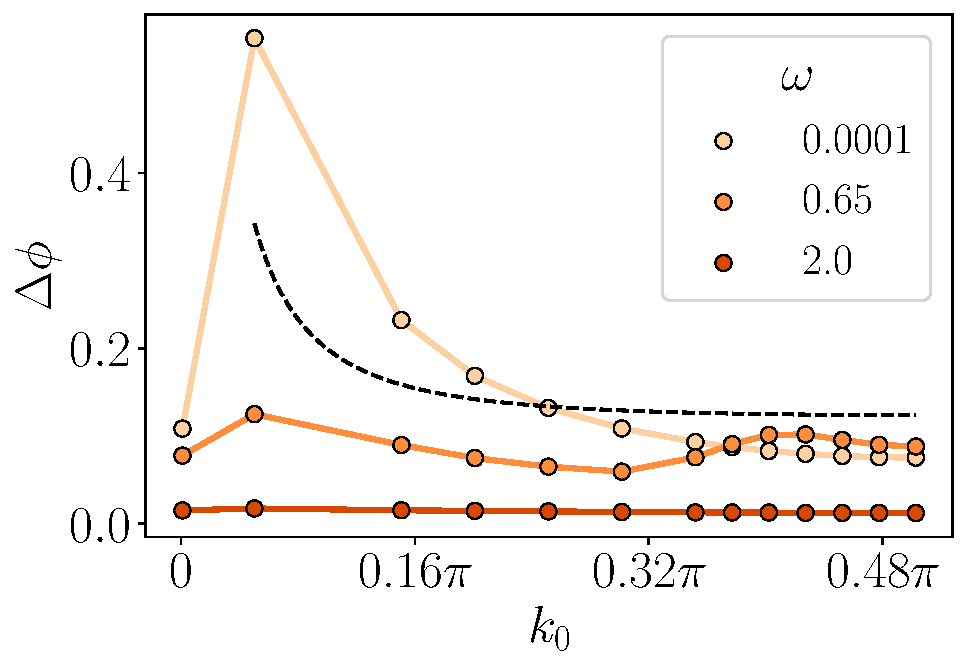
\includegraphics[width=0.55\linewidth]{Figures/phase_v_k0.pdf}%
    \label{fig:delta_phi_k0}
  }\\
  \subfloat[]{%
    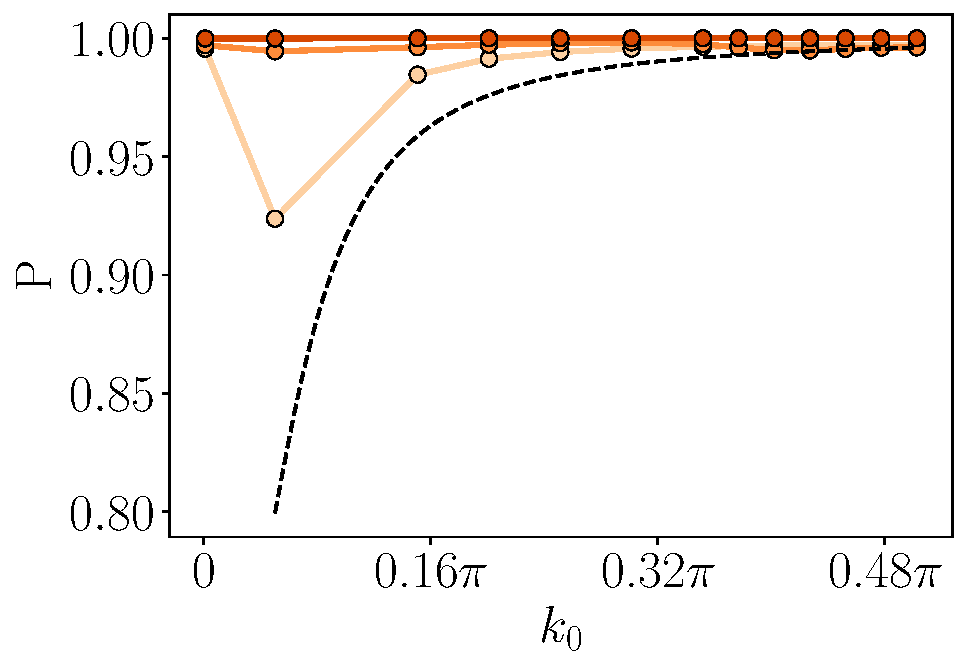
\includegraphics[width=0.55\linewidth]{Figures/purity_v_k0.pdf}%
    \label{fig:purity_k0}
  }
  \caption{Backaction on the qubit as a function of the central momentum $k_0$ for different Rabi frequencies $\omega$. The orange dots are data from exact diagonalization and the dashed line is the von Neuman analytical prediction from Eq.\eqref{eq:qubit_rho}. (a) Change in the qubit's phase due to measurement (b) Qubit's purity after measurement.}\label{fig:backaction_k0}
\end{figure}

\begin{itemize}
    \item These ED results can be understood with a toy model employing VN's approach \cite{romito2012} in the continuum limit.

    \item Before measurement, the dynamics are described by the free Hamiltonians of each independent system \cite{siddiqi2024}.
    
    \item At measurement, the time evolution operator is approximated by Eq.\eqref{eq:von_neumann_H} for small $\omega$ \cite{vonNeumann1932}.
    
    \item The resulting effective measurement strength $\tilde{g}=g\delta \tau$ depends on the time window $\delta\tau$.
    
    \item Applying Eq.\eqref{eq:von_neumann_H} results in an entangled state, coupling the $\ket{1}$ qubit state to the position of the wave packet (See \ref{app:derivation_backaction}). These are the so-called meter states \cite{svensson2013}.

    \item \sj{Maybe I should include the entangled state equation here}.
    
    \item Tracing out the detector yields the qubit's reduced density matrix Eq.\eqref{eq:qubit_rho} in terms of the new Bloch vector Eq.\eqref{eq:new_q}, valid to second order in $g$ \cite{siddiqi2024}.
    
    \item $\rho^{'}$ shows that the Rabi frequency remains unchanged and the qubit gains a phase $\Delta \phi (k_0)=-g k_0\delta \tau (k_0)$, where $\delta \tau$ is proportional to the spread of the wave-packet at the time of interaction (mentioned above).
    
    \item (\sj{discussion of the units may be necessary here})
    
    \item As mentioned, the change in phase is expected, since we break non-demolition.
    
    \item Purity is lost as $P=1/2 (1+R^2 \sin^2 (\theta_0) + \cos^2(\theta_0))$, with $R = e^{-g\delta \tau/4\Delta^2}$, consistent with dephasing measurement.

    \item The equations for $\Delta \phi$ and $k_0$ show that $k_0$ tunes the effective interaction strength by controlling the interaction time, in turn modifying $\tilde{g}$.

    \item Our results imply that, $k_0\rightarrow \pi/2$ to remain within the weak measurement regime . 

  \item VN fails to predict results for $\omega=0.65$ and $\omega=2.0$, however it evidences the role that $k_0$ plays  in defining the effective interaction strength.
   
    \item In the following, we situate the three observed behaviors in distinct entropy regimes, with a perturbative expansion.
\end{itemize}


\begin{align}\label{eq:von_neumann_H}
    \hat{U} = e^{-i g\delta \tau \hat{n}_1 \otimes \hat{p}},
\end{align}

\begin{align}\label{eq:qubit_rho}
    \rho_q^\prime = \frac{1}{2}(\id + \vec{q}^\prime \cdot \vec{\sigma})
\end{align}

\begin{align}\label{eq:new_q}
 \vec{q}^\prime = 
    \begin{pmatrix}
    R \sin(\theta_0) \cos(\phi + \Delta \phi(k_0)) \\
    R \sin(\theta_0) \sin(\phi + \Delta \phi(k_0)) \\
    \cos(\theta_0)
    \end{pmatrix}
\end{align}

\subsection{Entanglement Entropy}\label{sect:entanglement}

\begin{itemize}

\item The ED results in Fig.\ref{fig:entropy_phase_diagram} shows the post-measurement entropy as a function of both $k_0$ and $\omega$. It is normalized by the singlet entropy.

\item Highlight that entropy is an observable not discussed in the rate equation K,G formalism.

\item Three main regions: I. Scattering regime:  Entanglement constant in $\omega$. II. Coherent regime: entanglement exhibits a resonant line with enhanced entanglement. III. Floquet regime: Zero entropy, system and detector are decoupled.

\item Below the horizontal dashed green line, there is no weak measurement and the kick is ill defined. 

\item Appart from the final value of the entropy, each regime also has distinct time evolution (Fig.\ref{fig:entropy_time_evol}). 

\item Importantly, in region II (coherent), we see oscillations whenever the qubit crosses the $x$-$y$ plane on the bloch sphere

\item Despite these differences, the QPC transmission exhibits only a  slight change in its final value, indicating that the net result is an enhanced measurement strength.
\end{itemize}

\begin{figure*}
  \centering
  % --- Left: big figure ---
  \begin{minipage}{0.45\linewidth}
    \centering
    \subfloat[\label{fig:entropy_phase_diagram}]{%
      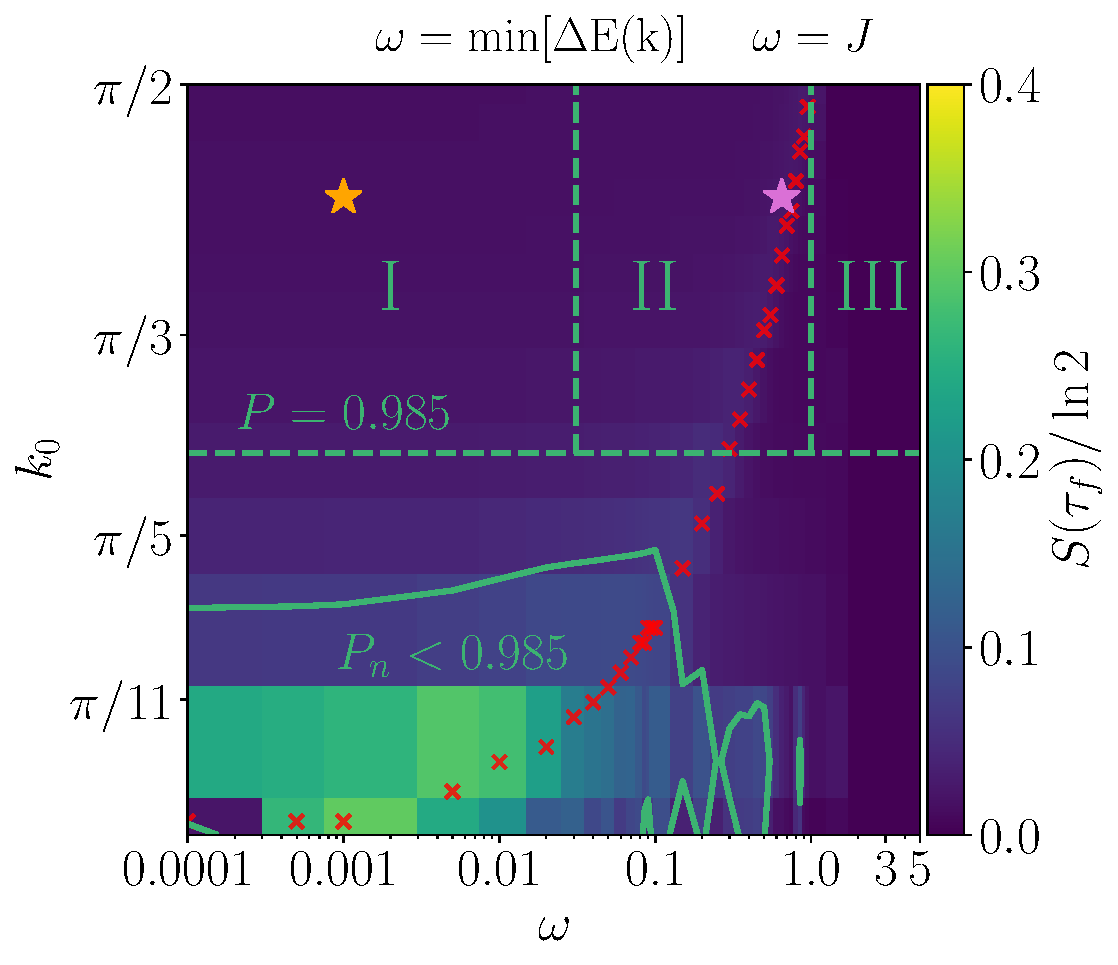
\includegraphics[width=\linewidth]{Figures/entropy_vs_K0_and_om.pdf}
    }
  \end{minipage}
  \hfill
  % --- Right: 2 small figures ---
  \begin{minipage}{0.46\linewidth}
    \centering
    \subfloat[\label{fig:entropy_time_evol}]{%
      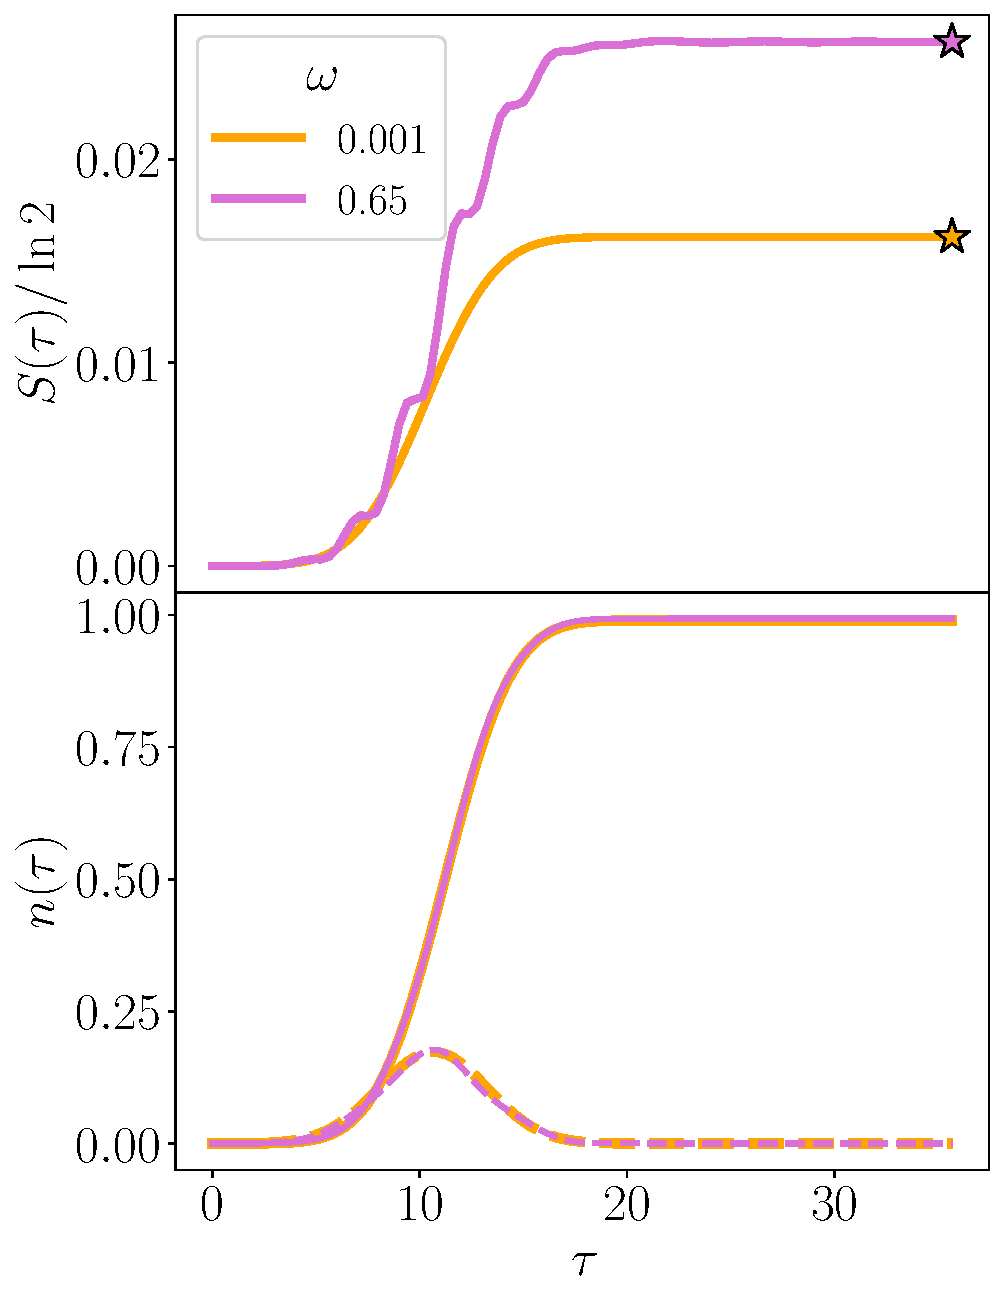
\includegraphics[width=0.55\linewidth]{Figures/compare_example.pdf}% 
      }
  \end{minipage}
  \caption{(a) Post-entanglement Entropy (Normalized by the singlet-entropy) as a function of wave-packet momentum and Rabi frequency. The dashed, green vertical lines bound the regimes according to Eq.\eqref{eq:entropy_bounds} and the dashed horizontal line marks where the purity from Eq.\eqref{eq:qubit_rho} falls below 0.985. The solid line indicates where the purity from the exact diagonalization $P_n$ falls bellow that same threshold. In addition, the red dots show the resonant line, where the qubit energy becomes degenerate with the QPC's kinetic energy. (b) \sj{add one for regime III} Top: Time evolution of the entanglement entropy. Bottom: Time evolution of the QPC transmission to the right of the bond (solid line) and the occupation directly at the bond (dashed line). The purple and orange lines are color coded to correspond to the points marked by stars in (a).}
\end{figure*}

\begin{widetext}
\begin{equation}
    \ket{\psi_\nu^{(1)} (k)} = \frac{1}{N+1} \sum_{p \neq k} \ket{p} \otimes \left\{\frac{\xi(k,p)}{-2J(\cos k - \cos p)} \ket{\nu} + \frac{\xi(k,p)}{2\epsilon_\nu - 2J(\cos k - \cos p)} \ket{\mu} \right\} + \frac{1}{N+1} \frac{\xi(k,k)}{2\epsilon_\nu} \ket{k} \otimes \ket{\mu}\label{eq:psi_first_order}
\end{equation}
\end{widetext}

\begin{subequations}\label{eq:entropy_bounds}
\begin{align}
    & \omega < \text{min}\Delta E (k) \\
    & \omega  > J  
\end{align}
\end{subequations}

\begin{itemize}
    \item The processes that dominate each of these regions are identified with each term in Eq.\eqref{eq:psi_first_order}. Derived in Appendix \ref{app:derivation_perturbative}.

    \item Specifically, we are are looking for processes that mix different bands \sj{Why can we do this? I think we can justify our interpretation in terms of scattering from the point of view of the S-matrix which should correspond to these three processes too}.

    \item The first term is similar to a tight binding model with constant external potential and is degenerate only towards the edges of the Brillouin zone (we are not interested in these). Mostly relevant to regime III in \ref{fig:entropy_phase_diagram}.
    
    \item Since it represents events where scattering happens only between states inside the same band, we have no entanglement. 

    \item The third term mixes between band gaps, but is only degenerate when the Rabi frequency approaches zero, therefore it only becomes relevant in regime I.

    \item Here, we have a scattering process between two bands without momentum exchange. Entropy production is influenced purely by the size of the time window.

    \item Finally, we have the second term which also mixes between two different bands ($\mu \neq \nu$). It is degenerate whenever the difference between two momenta is equal to the band gap.

    \item This is only possible inside regime II, as dictated by the bounds Eq.\eqref{eq:entropy_bounds} plotted in Fig.\ref{fig:entropy_phase_diagram}.

    \item The second term also shows that the resonant line corresponds to $2\epsilon_\nu = \Delta E(k)$ where the symmetric and anti-symmetric states are strongly hybridized. 

    \item The resonant line is a feature of the eigenenergies, but in our setup its only becomes relevant when $k_0$ crosses it. This explains the non-monotonic behavior in Fig.\ref{fig:backaction_k0}.

  \item \sj{One can thing of this in analogous terms to hydronic excitations. The difference is that, here the energy transfer goes to/from the qubit}

  \item \sj{This sort of transfer of energy through measurement has been observed in cotunneling \cite{zilberberg2014}}.

  \item We note that, the resonant line is not a finite size effect, but generic in large systems. In fact it is more pronounced in long chains: as momentum states become more dense, we will always find two whose energy difference is the same as the band gap.
\end{itemize}

\section{Discussion and Outlook}\label{sect:outlook}

\begin{itemize}
    \item We propose a simple Hamiltonian model for the QPC-qubit measurement process, that allows us to go beyond the typical treatment.

    \item Our model allows a well defined weak-measurement kick in terms of the width of a Gaussian wave packet and the post-measurement purity. 
    
    \item We show that the main parameters are $k_0$ and $\omega$, and ideintify their range.

    \item From the entanglement entropy and backaction on the qubit, we found 3 regimes: Static, coherent and Floquet, and identified the entropy generating processes via the degeneracies of the perturbative corrections.
        
    \item In the quasi-static regime, we reproduced the main features of non-invasive QPC measurements from VN, K and G: Our transition agreed with VN/Landauer and purity loss is consistent with dephasing in continuous measurements. \sj{Rabi change?}

    \item In this regime, entropy is generated when the symmetric and anti-symmetric states become degenerate.

    \item On the other hand, we show that in Floquet regime, the QPC and qubit become decoupled.

    \item This is reflected both in the backaction and the entropy. The later is explained by perturbative terms similar to a tight-binding chain interacting with an external, constant potential, which is only relevant for slow wavepackets (edges of Brillouin zone).
    
    \item Finally, the coherent regime exhibits unique behavior, characterized by a resonant line resulting in enhanced measurement strength.

    \item This resonant line indicates that more energy is absorbed/emitted by the system through a new scattering channel not present in typical calculations.

    \item \sj{Now follow up with Outlook ideas}
    
    \item \sj{Rabi frequency is constant so this can be a way of implementing robust phase gates}
        
    \item \sj{The phase change is also seen in \cite{jordan2008} and we could also extend our model to several subsequent measurements which could be used to prove Legget-Garg inequalities.}

    \item \sj{Another extension is including spin and valley degrees of freedom, relevant to sylicon based quantum computing}.

    
\end{itemize}

\section{RDM Statement}\label{sect:rdm}

\bibliographystyle{apsrev4-2} % APS recommended BibTeX style
\bibliography{qpc}     % Name of your .bib file (witho

% ---------------------------------------------------------------
% ---------------------------------------------------------------
% ---------------------------------------------------------------
% APPENDICES
% ---------------------------------------------------------------
% ---------------------------------------------------------------
% ---------------------------------------------------------------

\appendix 

\section{Numerical Setup and Finite Size Effects}\label{app:numerical_setup}

\begin{itemize}
    \item For our numerical simulations it is convenient to express the Hamiltonian Eq.\eqref{eq:qpc_dd_H} in terms of the computational basis Eq.\eqref{eq:comp_basis}.
    \item The term $\ket{\vec{j}}$ indicates a particle in the $j$-th site of the QPC chain, $\ket{q}=\ket{0},\ket{1}$ represents the qubit state as a double dot.
    \item As the composite state includes a Gaussian wave-packet in the QPC, the initial spread $\Delta$ has to be chosen such that the spread in momentum space $\Delta_p = \hbar/(\sqrt{2}\Delta)$ is strongly peaked around the central momentum $k_0$, for clearly defined trajectories \cite{shankar1994}. 
    \item This allows us to calculate the traveling time of the QPC particle with Ehrenfest's theorem $\tau = \langle \delta x \rangle/v_g$ where $\delta x$ is the distance (in terms of lattice spacing) and $v_g = 2J\sin{k_0}$ is the group velocity.
    \item With this relation we can choose the initial state (in Eq.\eqref{eq:initial_state}) of the qubit, so it is always in the same occupation (parametrized by $\theta_f$) when the QPC hits the interaction site, regardless of $v_g$ Eq.\eqref{eq:qubit_init_condition}.
    \item This condition also ensures that the qubit always traces the same Bloch sphere trajectory, oscillating between both poles.
    \item  In addition, Ehrenfest's theorem helps in avoiding reflection effects, stopping the simulations when the wavepacket hits the end of the chain.

\end{itemize}

\begin{align}\label{eq:comp_basis}
    \ket{\vec{j}}\otimes \ket{q} = \ket{0 0 \dots 010 \dots 0}\otimes \ket{q}
\end{align}

\begin{align}\label{eq:qubit_init_condition}
    & \alpha_0 = \cos(\theta_0/2)  \\
    & \beta_0 = -i\sin(\theta_0/2) \\
    & \theta_0/2 = -\theta_f/2 + \tau_B \omega \\
\end{align}

\begin{itemize}
    \item A standard ED time evolution algorithm was implemented in numpy, by applying the time evolution operator to the initial state in the diagonal basis to obtain the time evolved state $\ket{\Psi (\tau)}$. 
    \item  We track the occupations by applying the projectors Eq.\eqref{eq:projectors} to the composite state $\ket{\Psi(\tau)}$
    \item We also get the qubit's reduced density matrix $\hat{\rho}_q (\tau)$ by tracing out the detector states and obtain the purity $P(\tau) = \Tr{\hat{\rho}_q(\tau)}$ and von Neumann entropy $S(\tau) = -\Tr{\hat{\rho}_q(\tau) \log{\hat{\rho}_q(\tau)}}$.
    \item From $\hat{\rho}_q (\tau)$ we can obtain the backaction, however extracting the Bloch angles from the numerical density matrix is problematic. 
    \item To avoid issues, we estimate the change in phase from the law of cosines between a free Bloch vector $\vec{q}$ and the coupled one from ED $\vec{q}^\prime$ Eq.\eqref{eq:numerical_delta_phi}.
    \item For the final Rabi frequency we apply a fast-Fourier transform to the occupations, after the measurement.
    \item \sj{Include discussion about extending the qubit dynamics to get a better estimate?}.
    \item Fig.\ref{fig:rabi_freq} shows that the change in Rabi frequency is too small to differentiate from numerical error, so we deprecate it.
\end{itemize}

\begin{align}\label{eq:projectors}
    & \hat{\Pi}_j = \ket{\vec{j}}\bra{\vec{j}}\otimes\id_2 \\
    & \hat{\Pi}_q = \id_N\otimes\ket{q}\bra{q}
\end{align}

\begin{align}\label{eq:numerical_delta_phi}
    \cos(\Delta \phi) = \frac{|\vec{q}|^2 + \vec{q}^\prime|^2 - |\vec{q} -\vec{q}^\prime |}{2 \vec{q}| \vec{q}^\prime| }
\end{align}

\begin{figure}
    \centering
    \includegraphics[width=0.5\linewidth]{example-image-a}
    \caption{(a) Change in Rabi frequency as a function of $k_0$ for several values of $\omega$. }
    \label{fig:rabi_freq}
\end{figure}


\begin{itemize}
    \item The parameters for the simulations are: $\Delta \tau =$, $N=100$, $J=1$,$\Delta = 7$, $x_c = 30 $, $x_b=50$, $\theta_f = $, $g \in \{\}$, $k_0 \in \{\}$, $\omega \in \{\}$.
    \item We express our results in unis of $J$.
\end{itemize}


\section{Von Neumann's Measurement Scheme}\label{app:derivation_backaction}

Go into detail on the ancilla measurement scheme, and the calculation of the reduced density matrix from it
Explain how von Neumann relates to ancilla measurement and talk about meter states and such.
Mention the projective limit

\begin{itemize}
    \item For the quasi-static regime, von Neumann's measurement scheme is a toy model. 
    \item We represent the QPC particle as a free wave-packet, interacting with the qubit.
    \item Following \cite{siddiqi2024}, we separate in three intervals: Before the interaction, the interaction at $t=0$ and after the interaction.
    \item We assume an initial product state
    \item Before, and after the interaction, system and detector follow only their respective intrinsic Hamiltonians
    \item During the interaction, lasting $\delta \tau$, they evolve according to the entanglement Hamiltonian as.
\end{itemize}

\begin{align}
    \hat{U}(\delta \tau) = e^{\int_0^{\delta \tau} d \tau H_I}
\end{align}

\section{Derivation of the Perturbative Corrections}\label{app:derivation_perturbative}

Derivation of the first and second order corrections to the wave function, include the eigenstates and energies of the decoupled case. Discuss why we don't get corrections to the entropy or backaction.

\begin{figure}[t]
    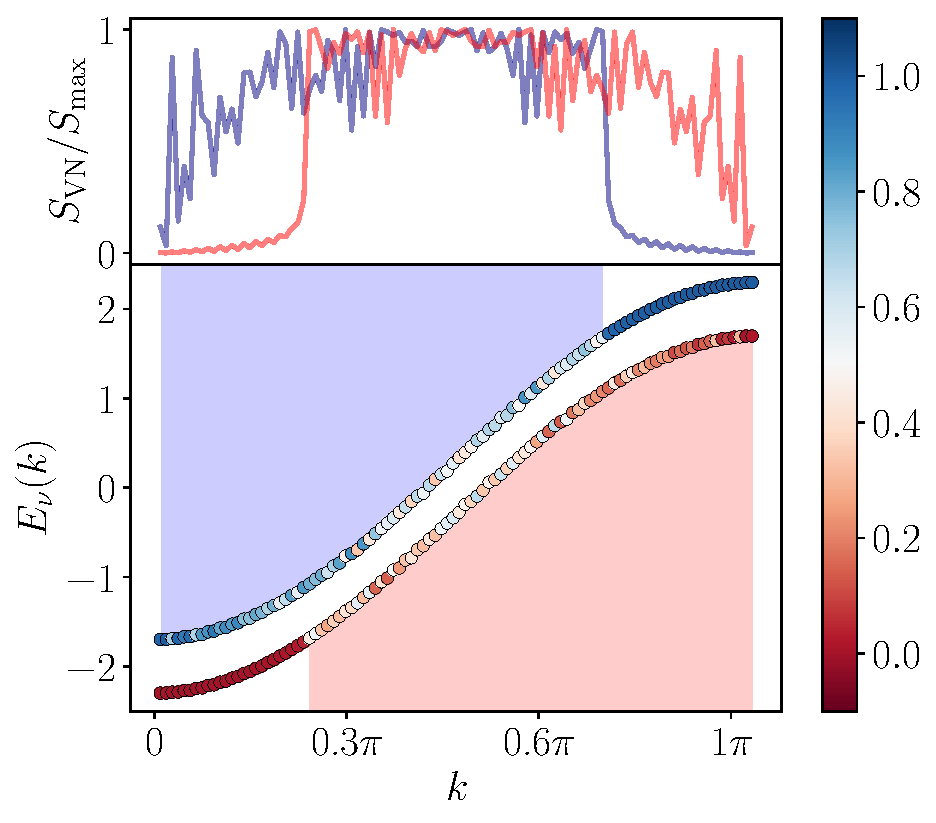
\includegraphics[width=0.7\linewidth]{Figures/exact_energies_Lqpc=100_Omega=1.0_t=0.3.pdf}
    \caption{Top: Entanglement entropy contributed by each eigenstate of the Hamiltonian. Bottom: Hybridization of the energy bands found via exact diagonalization. The color corresponds to the projection onto the symmetric state, the shaded regions indicate where each band becomes degenerate according to Eq. \eqref{eq:psi_first_order}.}
    \label{fig:entropy_spectrum}
\end{figure}



\end{document}
